\begin{figure}[!ht]
\centering
\resizebox{\linewidth}{!}{
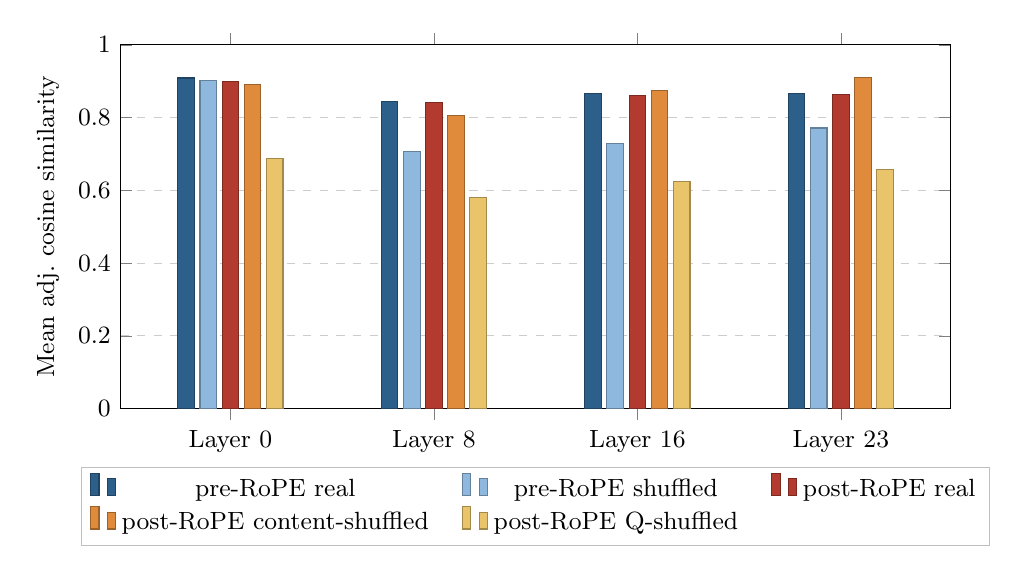
\begin{tikzpicture}
  \definecolor{preReal}{HTML}{2C5F8A}   % dark blue
  \definecolor{preShuf}{HTML}{8FB8DE}   % light blue
  \definecolor{postReal}{HTML}{B23A2E}  % dark red
  \definecolor{postCont}{HTML}{E08A3C}  % orange
  \definecolor{postShuf}{HTML}{E9C46A}  % light amber
  \begin{axis}[
    ybar,
    bar width=6pt,
    width=\textwidth,
    height=6.2cm,
    enlarge x limits=0.18,
    ymin=0, ymax=1,
    ytick={0,0.2,0.4,0.6,0.8,1.0},
    ylabel={Mean adj.\ cosine similarity},
    symbolic x coords={Layer 0, Layer 8, Layer 16, Layer 23},
    xtick=data,
    tick label style={font=\small},
    ylabel style={font=\small},
    ymajorgrids=true,
    grid style={dashed, gray!40},
    legend style={
      at={(0.5,-0.16)}, anchor=north,
      legend columns=3, font=\small,
      /tikz/every even column/.append style={column sep=10pt},
      draw=gray!50,
    },
  ]
    \addplot[fill=preReal,  draw=preReal!70!black]  coordinates {(Layer 0,0.9091) (Layer 8,0.8449) (Layer 16,0.8652) (Layer 23,0.8659)};
    \addplot[fill=preShuf,  draw=preShuf!70!black]  coordinates {(Layer 0,0.9010) (Layer 8,0.7075) (Layer 16,0.7281) (Layer 23,0.7716)};
    \addplot[fill=postReal, draw=postReal!70!black] coordinates {(Layer 0,0.9000) (Layer 8,0.8408) (Layer 16,0.8619) (Layer 23,0.8626)};
    \addplot[fill=postCont, draw=postCont!70!black] coordinates {(Layer 0,0.8922) (Layer 8,0.8047) (Layer 16,0.8736) (Layer 23,0.9114)};
    \addplot[fill=postShuf, draw=postShuf!70!black] coordinates {(Layer 0,0.6880) (Layer 8,0.5807) (Layer 16,0.6234) (Layer 23,0.6570)};
    \legend{pre-RoPE real, pre-RoPE shuffled, post-RoPE real, post-RoPE content-shuffled, post-RoPE Q-shuffled}
  \end{axis}
\end{tikzpicture}
}
\caption{Mean adjacent query cosine similarity per layer (averaged over all heads) for LLaMA-3.1 8B Instruct at layers 0, 8, 16, and 23, under five configurations: pre-RoPE real, pre-RoPE shuffled, post-RoPE real, post-RoPE content-shuffled, and post-RoPE Q-shuffled.}
\label{fig:query_similarity}
\end{figure}
